\documentclass{beamer}

\usepackage[T1]{fontenc}
\usepackage[swedish]{babel}
\usepackage{amssymb, graphicx}
\usepackage{beamerthemesplit}

\title{Customer Terminal}
\author{
	Emil Eriksson (c07een)\\
    Martin �slin (c07man)\\
    Johan Norberg (c07jng)\\
    Rickard Westerlund (c07rwd)\\
    Per Bj�rklund (c07pbd)\\
    Javid Jou (dv08dju)\\
}
\date{\today}

\begin{document}

	\frame{\titlepage}

	\frame{\tableofcontents}

	\section[Planning]{Planning}
	
		\subsection{Project management}
			\begin{frame}
			\begin{itemize}
			\item All written reports and presentations will be in English.
			\item For time tracking a spreadsheet in GoogleDocs will be used.
			\item Group meetings every week.
			\end{itemize}	
			\end{frame}

		\subsection{Tools and Methods}
			\begin{frame}
				\begin{itemize}
				\item Ruby using Ruby on Rails.
				\item SQLite database backend.
				\item HTML, CSS and JavaScript for user interface.
				\item Model-View-Controller design.
				\item Unit testing with Unit::TestCase.
				\item Metrics and code coverage with metric\_fu.
				\item GIT for version control.
				\end{itemize}
			\end{frame}

		\subsection{UML}
			\begin{frame}
				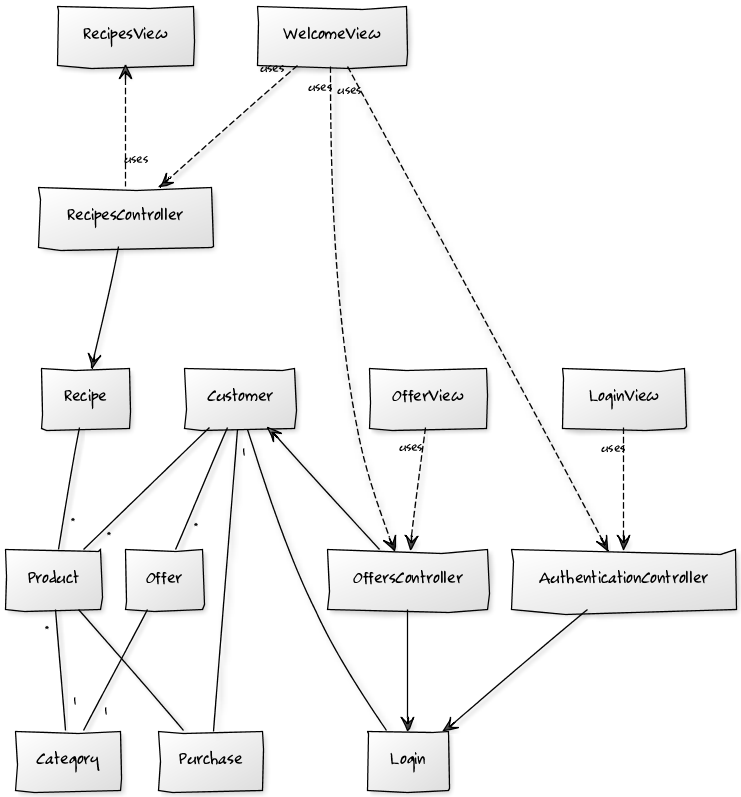
\includegraphics[scale=0.3]{images/uml.png}
			\end{frame}

		\subsection{GUI design}
			\begin{frame}
				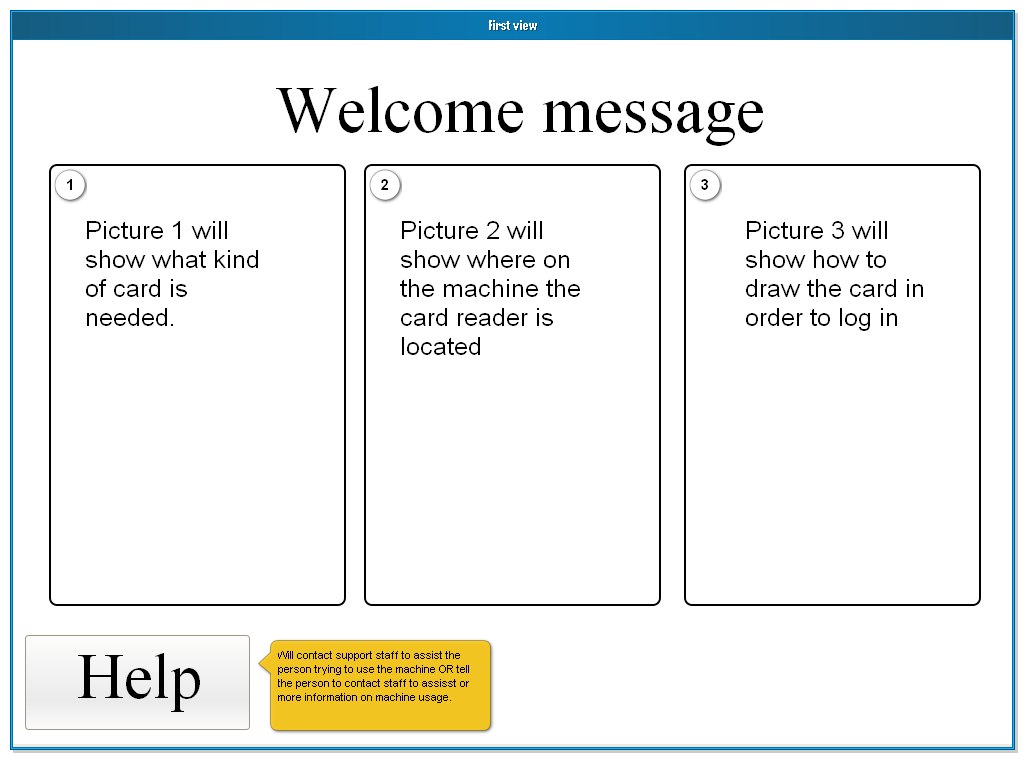
\includegraphics[scale=0.25]{images/gui/ica1.png}
			\end{frame}
			\begin{frame}
				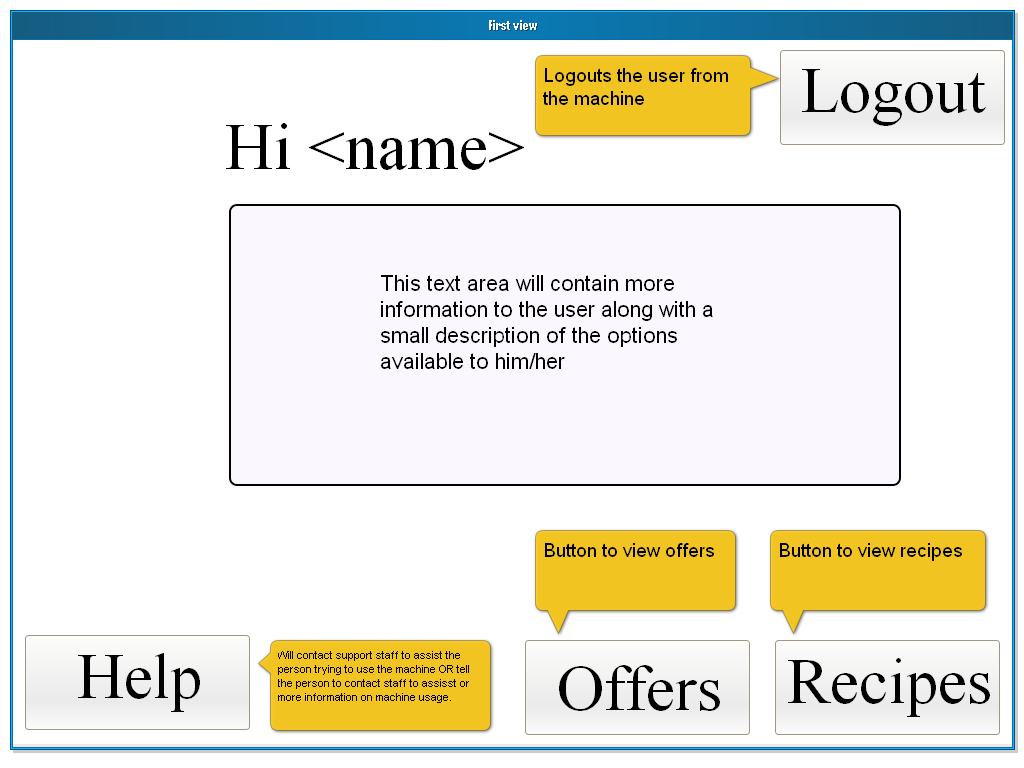
\includegraphics[scale=0.25]{images/gui/ica2.png}
			\end{frame}
			\begin{frame}
				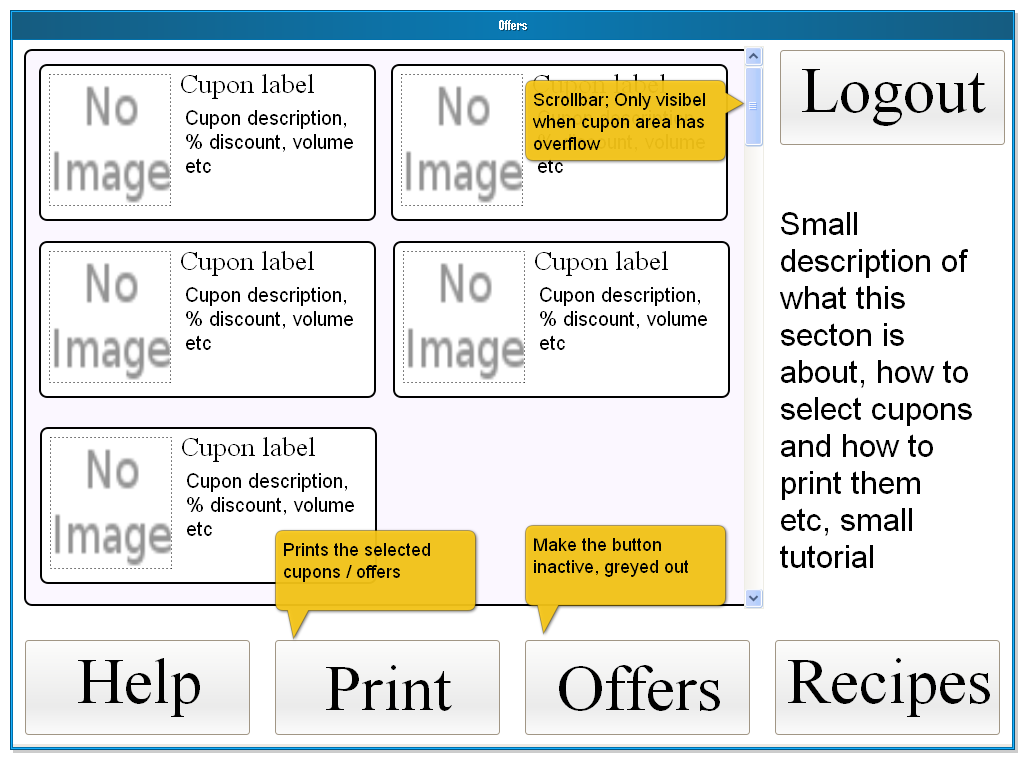
\includegraphics[scale=0.25]{images/gui/icaoffers.png}
			\end{frame}
			\begin{frame}
				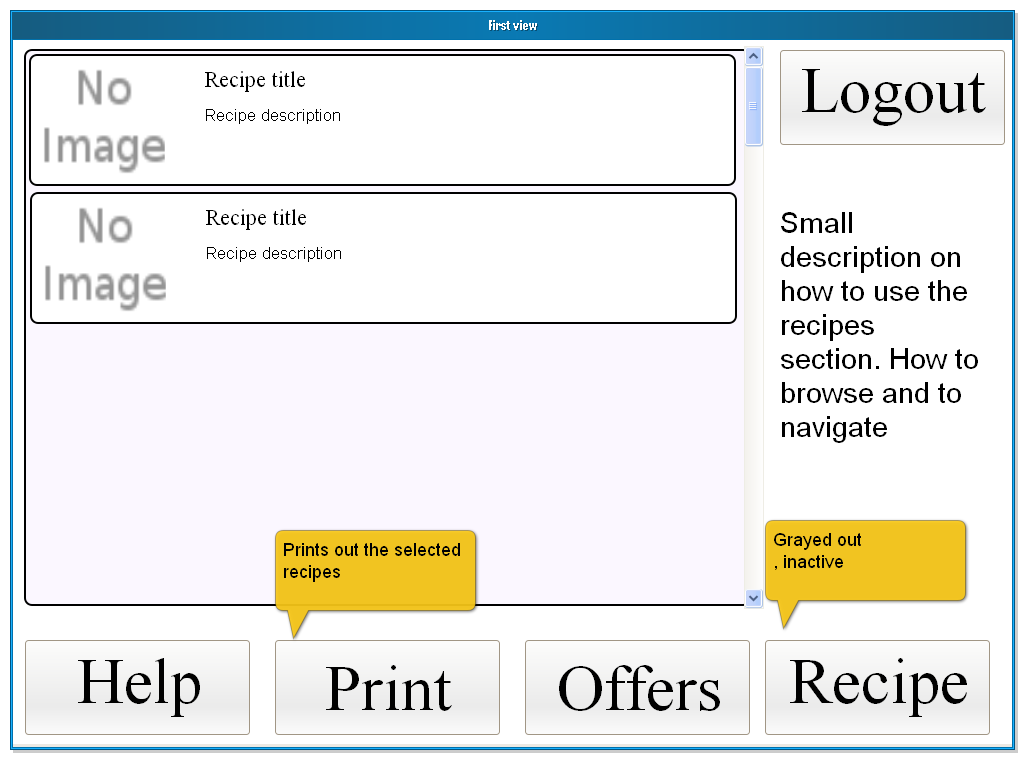
\includegraphics[scale=0.25]{images/gui/icarecipe.png}
			\end{frame}
		\subsection{Schedule and Milestones}
			\begin{frame}
				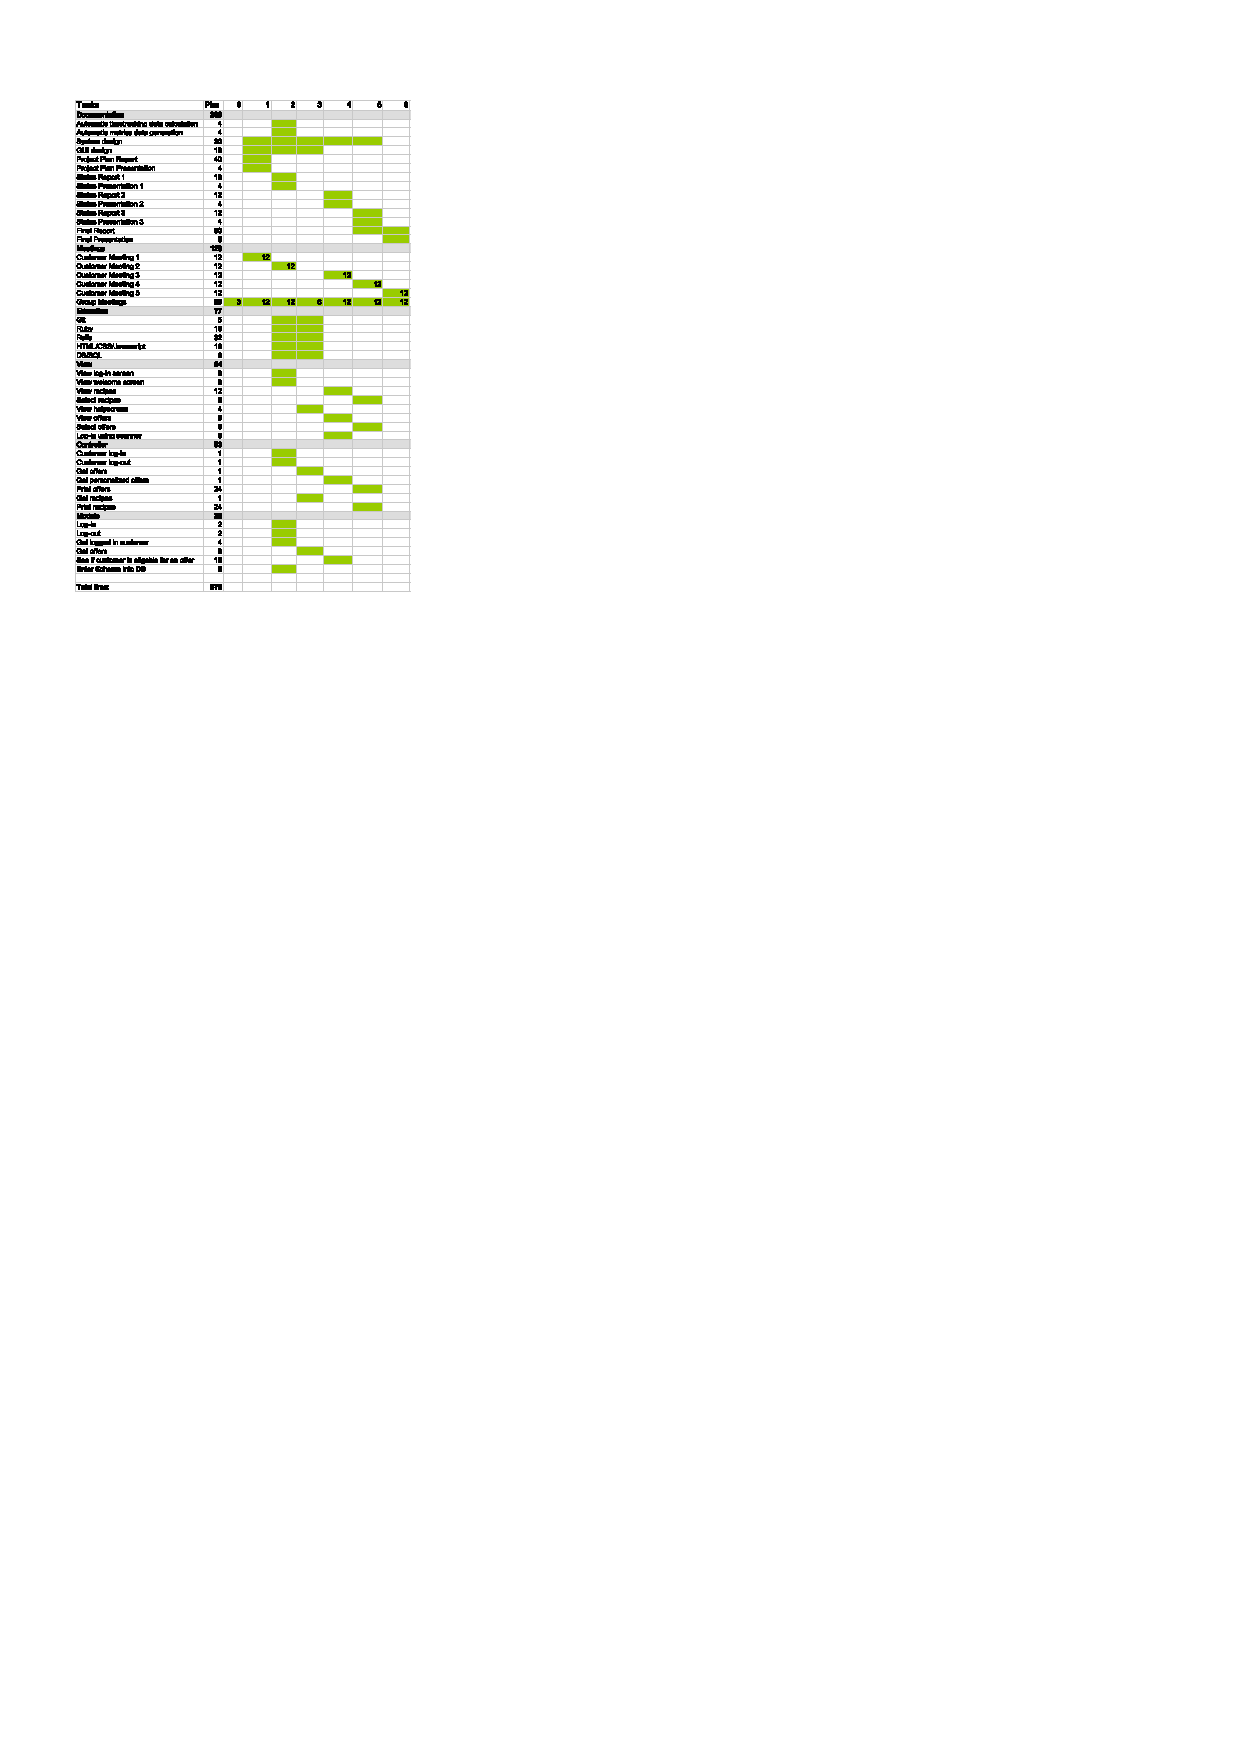
\includegraphics[scale=0.9]{images/schedule.pdf}
			\end{frame}

	\section[Quality Assurance]{Quality Assurance}
		\subsection{Accessibility}
			\begin{frame}
			\begin{itemize}
				\item Colorblindness
				\item Simplicity
				\item Visual impairment
			\end{itemize}
			\end{frame}

		\subsection{Metrics}
			\begin{frame}
			\begin{itemize}
				\item A code coverage of at least 90\%.
				\item An LCOM (defined by Henderson-Sellers) of no more than 0.6.
				\item Fan-In and Fan-Out values of no more than 5.
				\item Satisfy all the requirements in the specification.
			\end{itemize}
			\end{frame}

		\subsection[Risks]{Risks}
			\begin{frame}
			\begin{itemize}
				\item Little time with scanner.
				\item Little time with touch screen.
				\item Touch screen might not show up.
				\item Loss of team members.
				\item Conflicts
				\item Misinterpreted specification.
				\item Lack of experience with development tools.
				\item Testing GUI for a diverse customer base.
			\end{itemize}
			\end{frame}
\end{document}
